\documentclass[12pt,english]{scrartcl}

\usepackage{amsmath,amssymb}
%\usepackage[amssymb]{SIunits}
\usepackage{babel}
\usepackage[latin1]{inputenc}
\usepackage{graphicx}
\usepackage{color}
\usepackage{url}


\begin{document}

\begin{center}
\textbf{\begin{LARGE}KOGW-PM-KNP:\\ \vspace{3mm} Tutorial 10 - Spacing effects in learning
\end{LARGE}}
\end{center}

This tutorial deals with a strategies to optimize retention of learned material. The paper by Cepeda et al., (2008) conducts a large scale internet study and argue - based on their results - that many educational practices are highly inefficient. Please read the paper carefully. Answer the following questions which should help you to evaluate their findings. Please work in pairs. 
%  
% \begin{figure}[htbp]
% \begin{center}
% 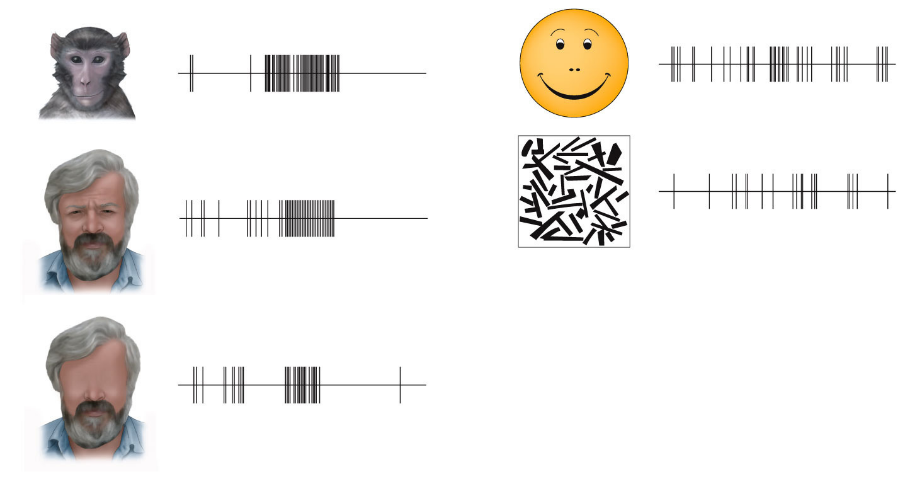
\includegraphics[width = 0.8\textwidth]{IT_cell.png}
% \end{center}
% \caption{
% \label{fig:IT_cell}}
% \end{figure}

\begin{enumerate}
 \item What was the research question addressed by the authors?

 \item Explain the typical design and result pattern of experiments on spacing effects or effects of distributed practice.

 \item What was reported in the study by Bahrick et al., 1993? What potential confound do the present authors identify in their study?

 \item What was the goal of the present study?

 \item Describe the procedure and the results of the preliminary study. Was that a within- or a between-subjects design, why?

 \item Describe the design and procedure of the main study.

\item The present results show that the timing of learning sessions can have powerful effects on retention when study time is equated. What is the major educational implication of this  result? Will that have an effect on your own study behavior?

 \item Describe the results of the main study.

\item List potential objections against Internet-based testing. Do you think the authors satisfactorily address the concerns?
 
\end{enumerate}

\end{document}
